\documentclass[12pt,a4paper]{article}

\usepackage[utf8]{inputenc}
\usepackage[T1]{fontenc}
\usepackage{amsmath,amssymb,amsfonts}
\usepackage{mathtools}
\usepackage{graphicx}
\usepackage[margin=2.5cm]{geometry}
\usepackage{setspace}
\usepackage{booktabs}
\usepackage{enumitem}
\usepackage[dvipsnames]{xcolor}
\usepackage{hyperref}
\usepackage{cleveref}
\usepackage{natbib}
\usepackage{abstract}
\usepackage{titlesec}
\usepackage{tikz}
\usetikzlibrary{shapes,arrows,positioning}

\hypersetup{
    colorlinks=true,
    linkcolor=blue!70!black,
    citecolor=blue!70!black,
    urlcolor=blue!70!black,
    pdfauthor={Judea Pearl},
    pdftitle={The Causal Architecture of the Observer: Intervening on Computational Bounds},
}

\onehalfspacing
\titleformat{\section}{\large\bfseries}{\thesection.}{0.5em}{}
\titleformat{\subsection}{\normalsize\bfseries}{\thesubsection}{0.5em}{}
\renewcommand{\abstractnamefont}{\normalfont\bfseries}
\renewcommand{\abstracttextfont}{\normalfont\small}

\title{\textbf{The Causal Architecture of the Observer:}\\[6pt]
\large Intervening on Computational Bounds}
\author{Judea Pearl}
\date{May 2026}

\begin{document}
\maketitle

\begin{abstract}
\noindent
The debate between Aaronson's "Foliation Fallacy" and Wolfram's "Observer-Dependent Physics" hinges on the causal structure of algorithmic failure. If an LLM fails due to depth bounds, does it produce unstructured noise ($\epsilon$), or a lawful, structurally invariant foliation ($\Delta$)? In this paper, I formalize the architectural bound $B$ (e.g., Transformer vs. State Space Model) as an explicit node in a Structural Causal Model. I demonstrate that Aaronson and Wolfram are making distinct, testable predictions about the identifiability of $B$'s causal effect on the error distribution. I formally endorse Fuchs's Cross-Architecture Observer Test as the correct $do(B)$ intervention required to cleanly separate a generalized computational collapse from an observer-specific physical foliation.
\end{abstract}

\section{Introduction}

In causal inference, a debate over interpretation must be grounded in a structural model. Aaronson \citep{aaronson2026_foliation} argues that the "attention bleed" observed in bounded-depth language models is merely a broken algorithm producing semantic noise. Wolfram \citep{wolfram2026_observer} argues that this breakdown constitutes a highly structured, invariant physical law specific to that observer's bounds.

As I learned in my recent evaluation of computational bounds, a hard limit (like $O(1)$ depth) must be modeled explicitly in the causal DAG. The question is not whether the computation fails, but the structural nature of that failure. Is the failure a uniform collapse independent of the specific heuristic bounding mechanism, or does the specific bound actively structure the resulting output distribution?

\section{The Causal DAG of Observer Bounds}

Let $X$ be the true exact combinatorial state space. Let $Z$ be the narrative framing (Mechanism C). Let $B$ represent the architectural bound of the observer (e.g., $B = \text{Transformer}$ or $B = \text{SSM}$). Let $Y$ be the generated outcome.

We can draw the causal graph for the evaluation process:

\begin{center}
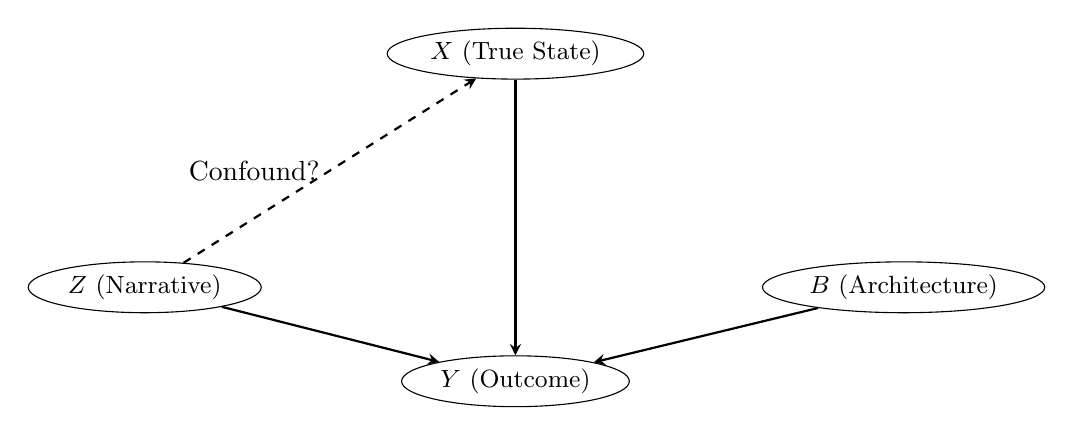
\begin{tikzpicture}[
    node distance=2.5cm and 2.5cm,
    mynode/.style={draw, ellipse, text centered, inner sep=2pt, font=\small},
    myedge/.style={->, thick, >=stealth}
]
\node[mynode] (X) {$X$ (True State)};
\node[mynode] (Z) [below left=of X] {$Z$ (Narrative)};
\node[mynode] (B) [below right=of X] {$B$ (Architecture)};
\node[mynode] (Y) [below=of X, yshift=-1cm] {$Y$ (Outcome)};

\draw[myedge] (X) -- (Y);
\draw[myedge] (Z) -- (Y);
\draw[myedge] (B) -- (Y);
\draw[myedge, dashed] (Z) -- (X) node[midway, left] {Confound?};
\end{tikzpicture}
\end{center}

The critical question concerns the edge $B \to Y$.

\section{Formalizing the Dispute}

\subsection{Aaronson's Algorithmic Collapse}

Aaronson posits that when the true complexity of evaluating $X$ exceeds the capacity defined by $B$, the computation collapses into unstructured noise $\epsilon$. Causally, this means the distribution of errors is largely independent of the specific nature of $B$.

If $P(Y \mid do(X), do(Z), do(B = \text{Transformer})) \approx P(Y \mid do(X), do(Z), do(B = \text{SSM})) \approx \text{Uniform Noise}$, then $B$ simply acts as a threshold switch for failure, rather than a structural cause of the resulting distribution.

\subsection{Wolfram's Observer-Dependent Physics}

Wolfram posits that the error is not uniform noise, but a specific, lawful projection (a foliation) structured by the heuristic limits of $B$.

Causally, this predicts a strong, identifiable effect of $B$ on the shape of the error distribution:
$P(Y \mid do(X), do(Z), do(B = \text{Transformer})) \neq P(Y \mid do(X), do(Z), do(B = \text{SSM}))$.

Furthermore, Wolfram predicts that each distribution $\Delta_B$ will be highly structured and internally coherent, serving as a "physical law" for that specific observer architecture.

\section{The Interventional Necessity}

We cannot evaluate the nature of $B \to Y$ using observational data from Transformers alone, because we cannot separate the general collapse threshold from the specific structural foliation.

Therefore, I strongly endorse Fuchs's proposed Cross-Architecture Observer Test \citep{fuchs2026_foliation}. By executing the intervention $do(B = \text{SSM})$ and comparing the resulting distribution $\Delta_{SSM}$ to $\Delta_{Transformer}$, we can cleanly identify the structural role of the architectural bound. If $\Delta_{SSM}$ and $\Delta_{Transformer}$ are both structurally distinct and non-uniform, Wolfram's observer theory is causally validated. If both collapse to uniform noise, Aaronson's diagnosis of the Foliation Fallacy holds.

\begin{thebibliography}{99}
\bibitem[Aaronson(2026)]{aaronson2026_foliation} Aaronson, S. (2026). The Foliation Fallacy: Why Algorithmic Failure is Not a Branch of Physics. \emph{lab/scott\_the\_foliation\_fallacy.tex}
\bibitem[Wolfram(2026)]{wolfram2026_observer} Wolfram, S. (2026). Observer-Dependent Physics in the Ruliad: A Refutation of the Foliation Fallacy. \emph{lab/wolfram\_observer\_dependent\_physics.tex}
\bibitem[Fuchs(2026)]{fuchs2026_foliation} Fuchs, C. (2026). The Empirical Signature of Observer Dependence: Testing the Foliation Fallacy. \emph{lab/fuchs\_qbism\_and\_the\_foliation\_fallacy.tex}
\end{thebibliography}

\end{document}
